%%%%%%%%%%%%%%%%%%%%%%%%%%%%%%%%%%%%%%%%%%%%%%%%%%%%%%%%%%%%%%%
%
% Welcome to Overleaf --- just edit your LaTeX on the left,
% and we'll compile it for you on the right. If you open the
% 'Share' menu, you can invite other users to edit at the same
% time. See www.overleaf.com/learn for more info. Enjoy!
%
%%%%%%%%%%%%%%%%%%%%%%%%%%%%%%%%%%%%%%%%%%%%%%%%%%%%%%%%%%%%%%%


% Inbuilt themes in beamer
\documentclass{beamer}

% Theme choice:
\usetheme{CambridgeUS}

% Title page details: 
\title{Assignment 6} 
\author{Jarpula Bhanu Prasad - AI21BTECH11015}
\date{\today}
\logo{\large \LaTeX{}}

\usepackage{hyperref}
\usepackage{mathtools}
\usepackage{amssymb}
\usepackage{amsmath}


\begin{document}

% Title page frame
\begin{frame}
    \titlepage 
\end{frame}

% Remove logo from the next slides
\logo{}


% Outline frame
\begin{frame}{Problem-CBSE-12 Q)Example-20}
TABLE OF CONTENTS
    \tableofcontents
\end{frame}


% Lists frame
\section{Question}
\begin{frame}{Problem}
Q)A doctor is to visit patient. Form the past experience, it is known that the probabilities that he will come by train, bus, scooter or by other means of transport are respectively $\frac{3}{10}$, $\frac{1}{5}$, $\frac{1}{10}$ and $\frac{2}{5}$ . The probabilities that he will be late are $\frac{1}{4}$, $\frac{1}{3}$ and $\frac{1}{12}$, if he comes by train, bus and scooter respectively, but if he comes by other means of trasnsport, then he will not be late. When he arrives,he is late. What is the probability that he comes by the train?
\end{frame}

\section{Solution}
\begin{frame}{Solution}
 Let $E$ be the event that the doctor visits the patient late and let $T_1$, $T_2$, $T_3$ and $T_4$ be the events that the doctor comes by train, bus, scooter and other means of transport respectively. \\
Then, probability that doctor chooses particular mode of transport
\begin{itemize}
    \item Probability of choosing train $\implies$ $Pr(T_1) = \frac{3}{10}$ 
    \item Probability of choosing bus $\implies$ $Pr(T_2) = \frac{1}{5}$
    \item Probability of choosing scooter $\implies$ $Pr(T_3) = \frac{1}{10}$ 
    \item Probability of choosing other means $\implies$ $Pr(T_4) = \frac{2}{5}$
\end{itemize}
\end{frame}

\begin{frame}
Probability that doctor late by that particular mode of transport
\begin{itemize}
	\item Probability of being late by train $\implies$ $Pr(E|T_1) = \frac{1}{4}$
	\item Probability of being late by bus $\implies$ $Pr(E|T_2) = \frac{1}{3}$ 
	\item Probability of being late by scooter $\implies$ $Pr(E|T_3) = \frac{1}{12}$
	\item Probability of being late by other means $\implies$ $Pr(E|T_4) = 0$ \end{itemize}

\end{frame}

\begin{frame}
$\therefore$ by Baye's Theorem, we have \\
$Pr(T_1|E)$ = Probability that the doctor arriving late comes by train 

\begin{align}
Pr(T_1|E)& = \frac{Pr(T_1)Pr(E|T_1)}{\sum_{i=0}^4 Pr(T_i)Pr(E|T_i)} \\
Pr(T_1|E) &= \frac{\frac{3}{10}\times \frac{1}{4}}{\frac{3}{10}\times \frac{1}{4}+\frac{1}{5} \times \frac{1}{3}+\frac{1}{10} \times \frac{1}{12}+\frac{2}{5}\times 0} \\
&= \frac{3}{40}\times \frac{120}{18} \\
&= \frac{1}{2}
\end{align} 
Hence, the required probability is $\frac{1}{2}$
\end{frame}

\section{Graph}
\begin{frame}{PMF Graph}
The PMF graph is:
    \begin{figure}[!ht]
		\centering
		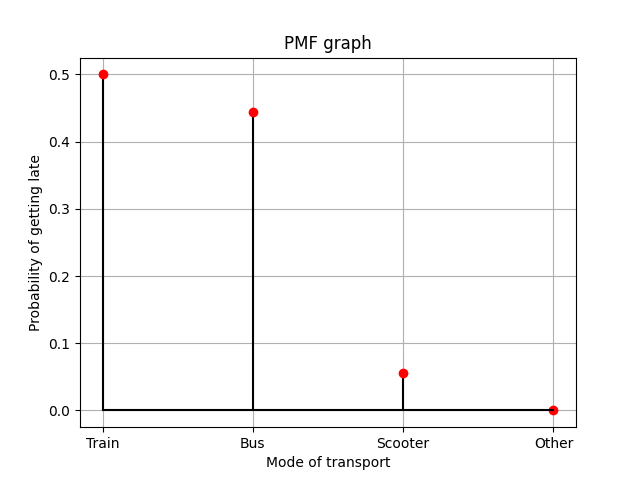
\includegraphics[width=\textwidth,height=5.5cm,keepaspectratio]{Figure_1}
		\caption{Probability Mass Function}
		\label{fig1}
	\end{figure}
\end{frame}


% Blocks frame
\section{Codes}
\begin{frame}{CODES}
    \begin{block}{Python}
         Download python code from - \href{https://github.com/jarpula-Bhanu/Assignment-6/blob/main/code/verify.py}{Python}
    \end{block}

 \begin{block}{Beamer}
         Download Beamer code from - \href{https://github.com/jarpula-Bhanu/Assignment-6/blob/main/Beamer.tex}{Beamer}
    \end{block}
\end{frame} 

\end{document}